\documentclass[11pt,a4paper]{article}
\usepackage[T1]{fontenc}
\usepackage[utf8]{inputenc}
\usepackage[french]{babel}
\usepackage{lmodern,microtype}
\usepackage[a4paper,margin=2.3cm]{geometry}
\usepackage{xcolor,graphicx,booktabs,tabularx,float,amsmath}
\usepackage{hyperref}
\usepackage[backend=biber,style=authoryear,sorting=nyt,maxbibnames=99]{biblatex}
\addbibresource{references.bib}
\definecolor{projectblue}{HTML}{153A5B}
\definecolor{projectcyan}{HTML}{168AAD}
\hypersetup{colorlinks=true,linkcolor=projectblue,citecolor=projectblue,urlcolor=projectcyan}

\title{\textcolor{projectblue}{Projet PI\textsuperscript{2} n\textsuperscript{o} 176}\\
\Large Dynamic of RND and Forecasting the Price of Derivatives\\[0.5em]
\large Rapport d'avancement n\textsuperscript{o} 1}
\author{Rayan Ait Arkoub, Matthieu Balliste, Ilan Chahdi,\\Nathan Denoux et Jordi Paris}
\date{20 octobre 2026}

\begin{document}
\maketitle

\begin{abstract}
Le projet vise à construire des séries temporelles de distributions risque-neutre
à partir d'options, à comparer trois méthodes d'estimation, à modéliser la dynamique
des densités et à évaluer une application à la couverture. Ce premier rapport fixe
le périmètre SPX, documente l'accès aux données et présente un prototype complet
Breeden--Litzenberger. Une photographie publique Cboe du 16 octobre 2026 fournit
1 446 contrats d'échéance 15 janvier 2027. Après nettoyage, 1 277 cotations sont
retenues et 338 points servent à calibrer une smile SVI à cinq paramètres. Le calcul
de densité est reproduit indépendamment en Python et en Julia.
\end{abstract}

\section{Problématique et objectifs}
Une volatilité Black--Scholes unique ne reproduit pas simultanément l'ensemble des
prix d'options d'une même échéance. L'existence d'un smile implique de travailler
avec une distribution risque-neutre commune à toute la coupe de strikes, plutôt
qu'avec un ajustement indépendant par option. Les étapes du projet sont la collecte
des données, l'estimation de trois RND, l'étude de leur stabilité, la prévision de
leur dynamique et l'utilisation de cette prévision dans une stratégie de couverture.

\section{Cadre théorique}
Pour une option européenne, un taux déterministe et un facteur d'actualisation
$D(t,T)$, le prix d'un call vérifie
\[
C_t(K,T)=D(t,T)\,\mathbb{E}^{\mathbb{Q}}[(S_T-K)^+].
\]
Sous des conditions de régularité, le résultat de \textcite{breeden_litzenberger_1978}
donne
\[
q_t(K,T)=\frac{1}{D(t,T)}\frac{\partial^2 C_t(K,T)}{\partial K^2}.
\]
La double dérivation amplifie le bruit de marché. Nous l'appliquons donc à une
courbe lissée et non aux derniers prix bruts, conformément aux recommandations de
\textcite{figlewski_2010} et à l'illustration du \textcite{bsic_2026}.

\section{Données et accès}
L'accès à l'API publique différée de Cboe est confirmé. Bloomberg n'est pas
accessible depuis l'environnement de développement actuel : aucun terminal ni API
locale n'est disponible. Il faudra réaliser l'export historique depuis un poste de
l'école ou obtenir OptionMetrics/Cboe DataShop. L'API publique permet néanmoins de
valider le pipeline sur une coupe réelle.

\begin{table}[H]
\centering
\begin{tabular}{lr}
\toprule
Horodatage & 16 octobre 2026, 17:12:17 \\
Spot SPX & 7 682,18 \\
Échéance sélectionnée & 15 janvier 2027 \\
Maturité & 91 jours \\
Contrats avant filtres & 1 446 \\
Cotations valides & 1 277 \\
Strikes call-put appariés & 362 \\
Points de calibration & 338 \\
\bottomrule
\end{tabular}
\caption{Description de l'échantillon initial.}
\end{table}

Le nettoyage privilégie le mid bid-ask, exclut les bids nuls, marchés croisés,
spreads relatifs supérieurs à 35\,\% et strikes excessivement éloignés. L'heure du
dernier échange est conservée comme diagnostic de staleness, mais le dernier prix
n'est pas utilisé lorsqu'un mid exploitable existe.

\begin{figure}[H]
\centering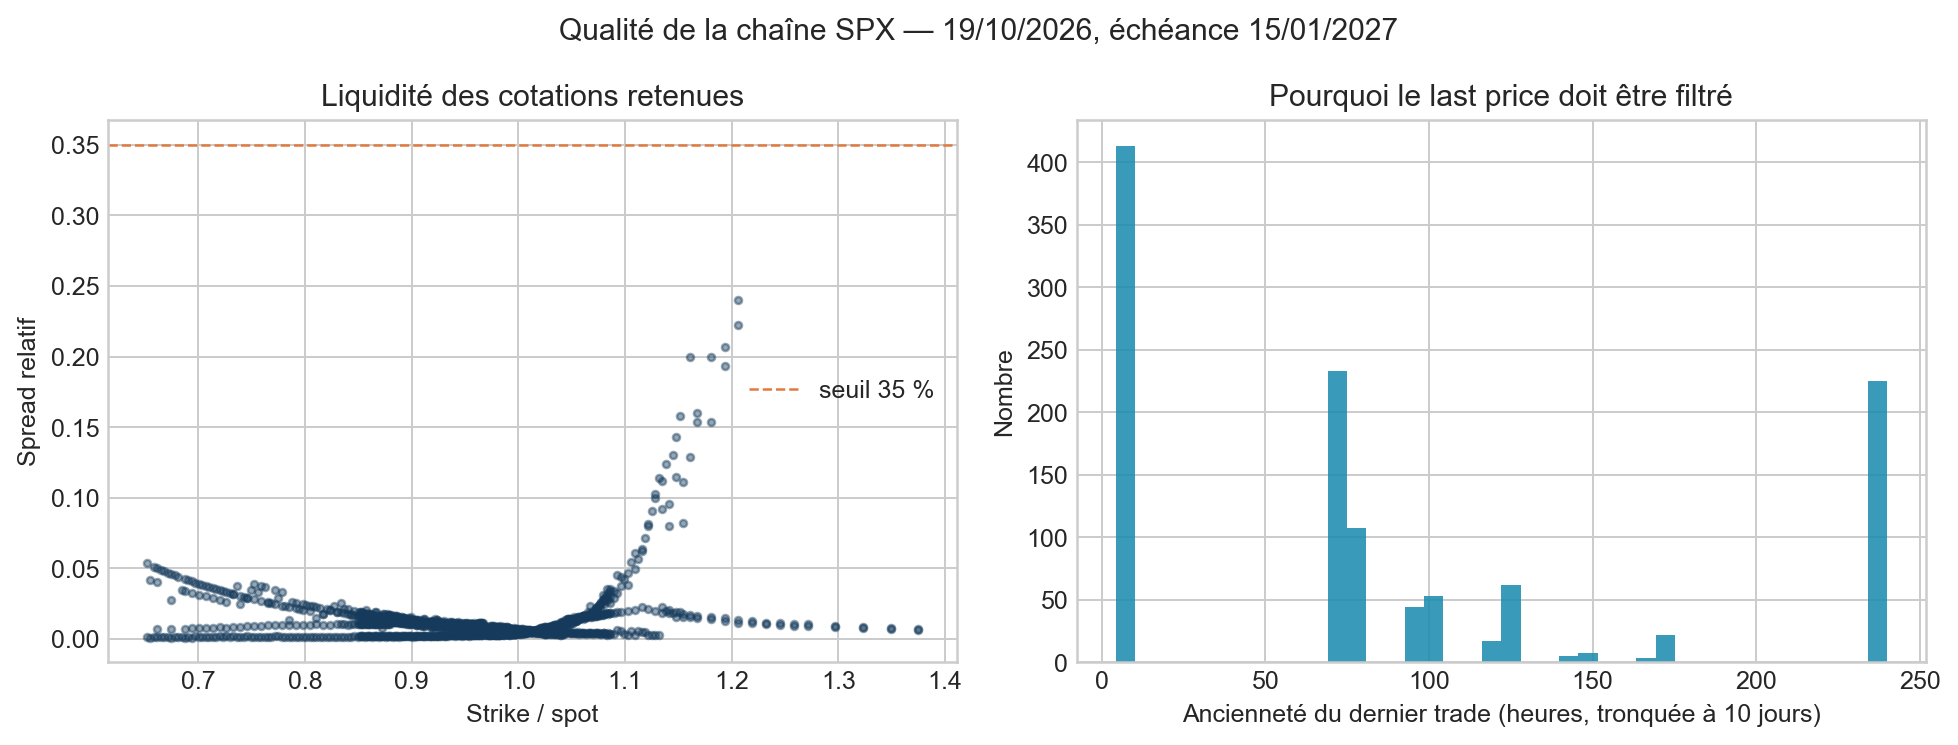
\includegraphics[width=0.95\textwidth]{results/01_data_quality.png}
\caption{Qualité des cotations et ancienneté des derniers échanges.}
\end{figure}

\section{Méthodologie du prototype}
Le forward $F$ et le facteur d'actualisation $D$ sont estimés conjointement par une
régression pondérée de la parité call-put $C-P=D(F-K)$ autour de la monnaie. Les
options hors de la monnaie sont ensuite utilisées pour construire des prix de calls
synthétiques : calls au-dessus du forward et puts transformés par parité en dessous.

Les volatilités implicites sont converties en variance totale et une SVI brute à
cinq paramètres est calibrée :
\[
w(k)=a+b\left[\rho(k-m)+\sqrt{(k-m)^2+\sigma^2}\right],\qquad k=\log(K/F).
\]
Cette paramétrisation fournit une coupe commune lisse. Les calls sont reconstruits
sur une grille régulière, puis dérivés deux fois. Le même calcul de différences
finies, normalisation, masse et moments est exécuté en Julia sans package externe.

\begin{figure}[H]
\centering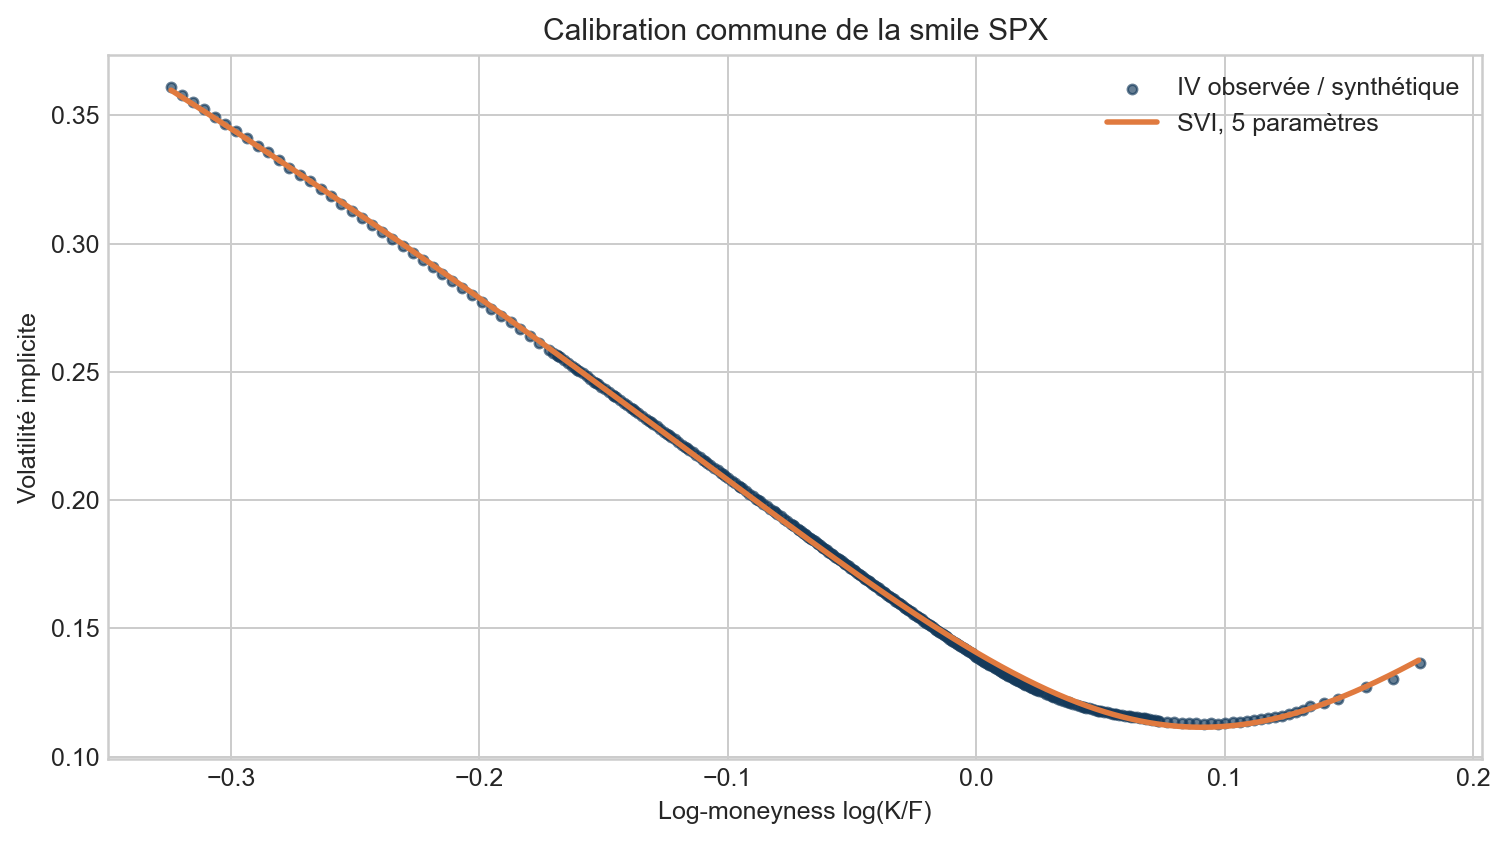
\includegraphics[width=0.82\textwidth]{results/02_svi_smile.png}
\caption{Volatilités implicites et calibration SVI à cinq paramètres.}
\end{figure}

\section{Premiers résultats}
La parité fournit $F=7\,755{,}89$, $D=0{,}98837$ et un taux continu implicite de
4,69\,\%. La RMSE de parité vaut 0,118 point d'indice. Les paramètres SVI estimés
sont $a=-0{,}02923$, $b=0{,}12073$, $\rho=-0{,}05133$, $m=0{,}08167$ et
$\sigma=0{,}26829$. La RMSE de reconstruction des calls est de 1,144 point.

\begin{figure}[H]
\centering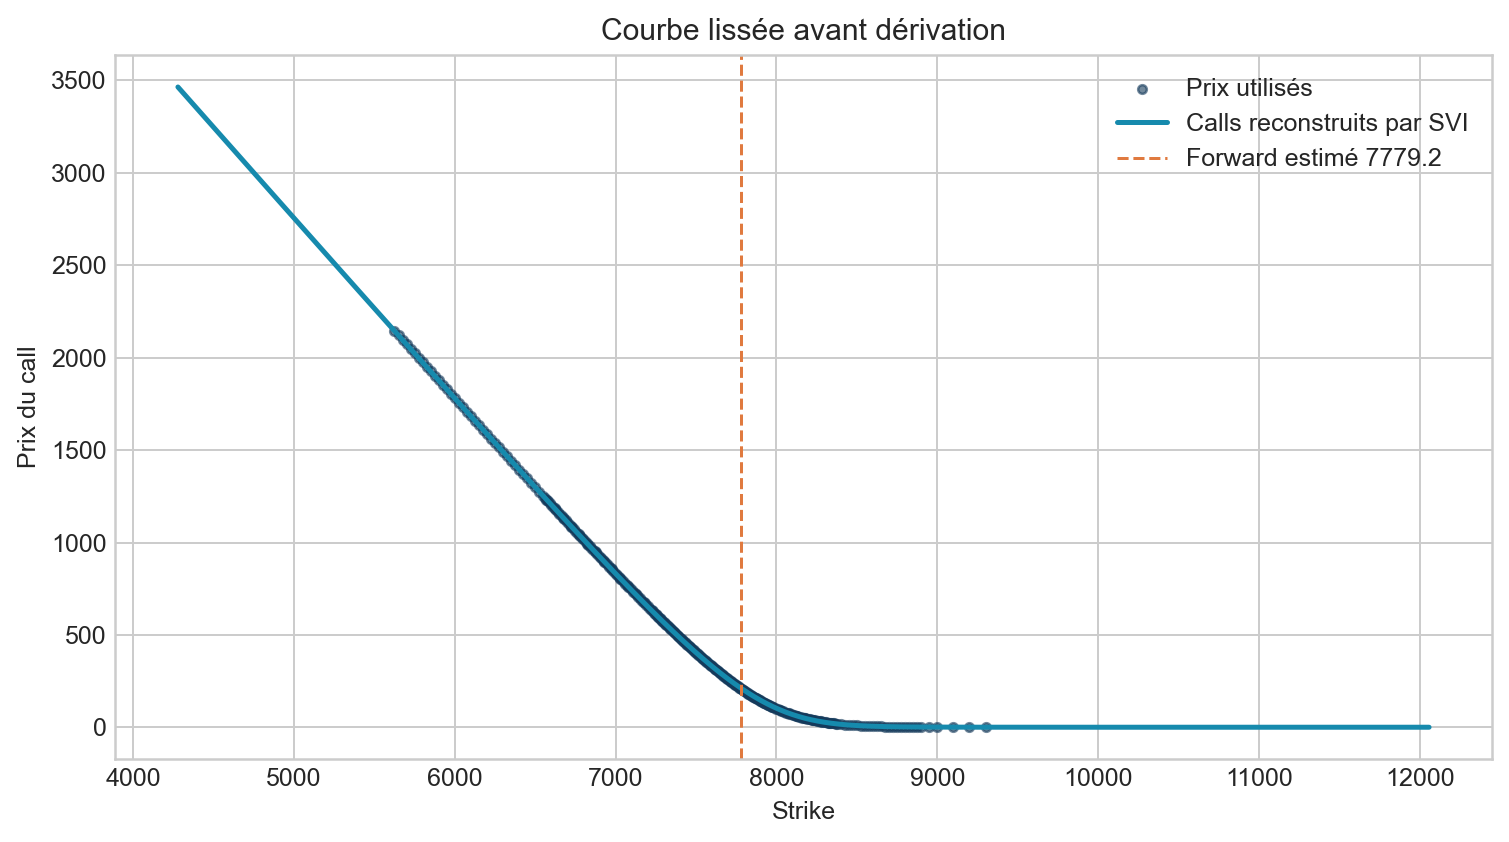
\includegraphics[width=0.82\textwidth]{results/03_call_curve.png}
\caption{Prix utilisés et courbe de calls reconstruite.}
\end{figure}

La masse brute de la densité sur la grille est 0,99528. Après suppression des seules
valeurs négatives et renormalisation, sa moyenne vaut 7 776,20. La masse négative
totale n'est que de 0,000117. Environ 20\,\% des points de l'extrême queue droite
sont légèrement négatifs, mais aucun n'est inférieur à $-0,1\,\%$ du pic de densité.
Cette distinction évite de présenter un pourcentage de points trompeur sans mesurer
l'amplitude économique de l'erreur.

\begin{figure}[H]
\centering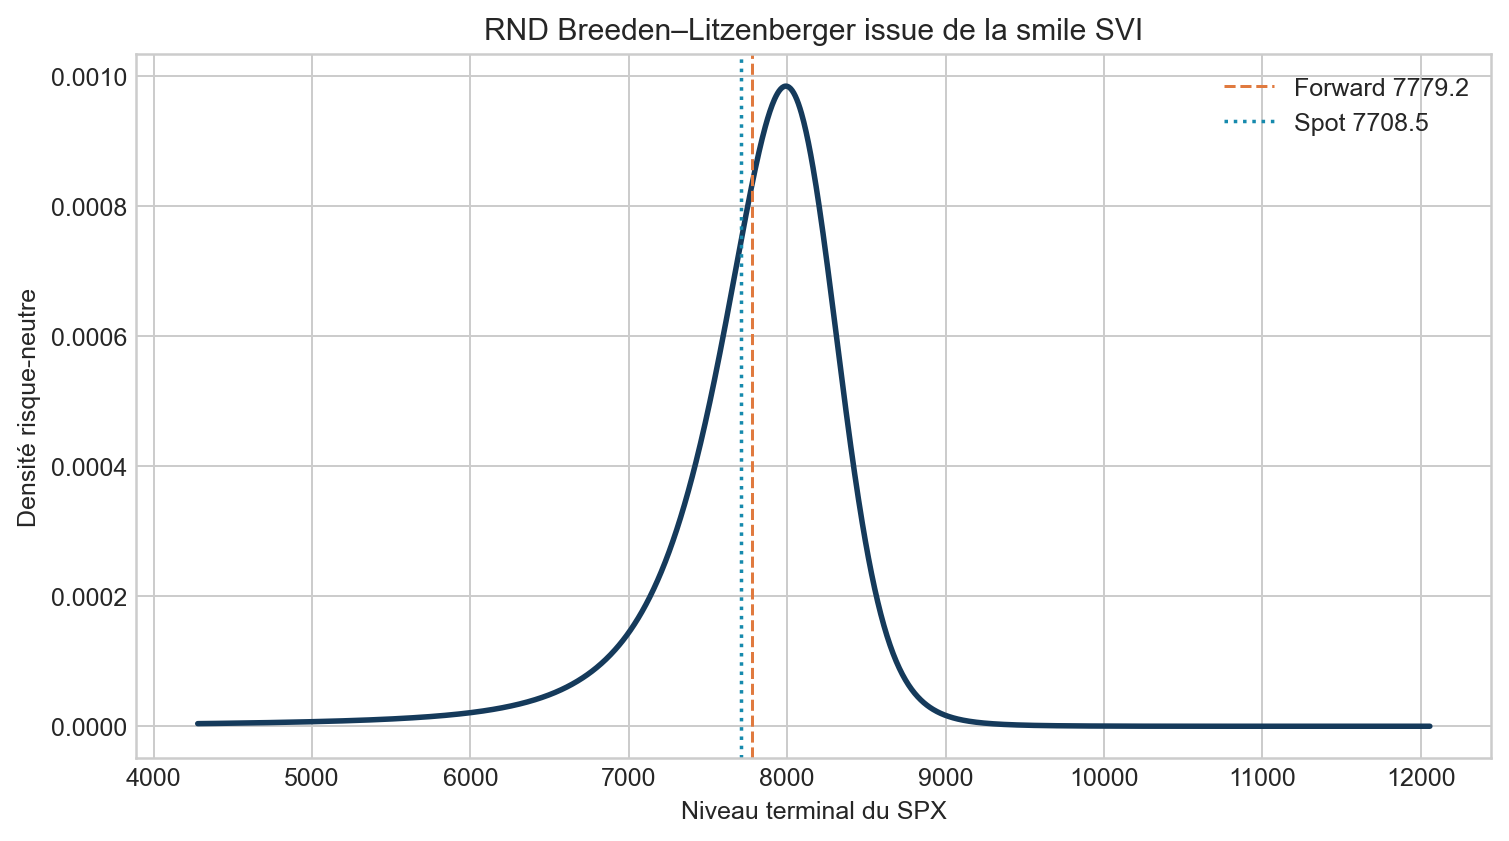
\includegraphics[width=0.82\textwidth]{results/04_risk_neutral_density.png}
\caption{Première densité risque-neutre SPX estimée par Breeden--Litzenberger.}
\end{figure}

Les résultats Julia et Python concordent : l'écart absolu moyen entre les densités
normalisées est de $3,3\times10^{-9}$ ; l'écart maximal, situé aux bords où les
schémas de dérivation diffèrent, est de $2,1\times10^{-6}$.

\section{Limites}
La photographie Cboe n'est pas une base historique. Le filtre de spread à 35\,\%
est provisoire et doit faire l'objet d'une analyse de sensibilité. La SVI brute
n'impose pas à elle seule toutes les contraintes d'absence d'arbitrage butterfly ;
la très faible négativité observée dans la queue doit être traitée ultérieurement
par une calibration sans arbitrage ou un lissage directement convexe des calls.
Enfin, la comparaison temporelle exigera une maturité constante ou une interpolation
entre deux échéances, afin de ne pas confondre dynamique et passage du temps.

\section{Suite du projet}
La prochaine étape consiste à obtenir un historique quotidien, appliquer les trois
méthodes de la fiche projet sur une grille commune de log-moneyness, puis comparer
les densités par entropie relative et distances robustes. Leur dimension sera réduite
par facteurs fonctionnels selon \textcite{giacomini_et_al_2009}. Les scores seront
modélisés par AR/VAR et évalués hors échantillon. L'incertitude sera étudiée dans
l'esprit de \textcite{taboga_2016}. Enfin, une couverture utilisant la RND prévue
sera comparée à un benchmark Black--Scholes en erreur de couverture nette de coûts.

\section{État des livrables}
Le dépôt contient le snapshot brut, deux tables traitées, un pipeline Python,
un calcul Julia autonome, les diagnostics JSON/texte, quatre figures et un script
PowerShell de reproduction. Le principal blocage externe demeure l'accès à une
profondeur historique suffisante.

\printbibliography[title={Références}]
\end{document}
